
\chapter{Sprint 4 : Implémentation des tableaux de bord }

\section*{Introduction}

Dans ce chapitre, nous détaillerons les étapes et processus de l'implémentation des tableaux de bord durant le sprint 4 de notre projet. Ces tableaux de bord, essentiels pour une visualisation claire des données, facilitent la prise de décisions éclairées pour les différentes parties prenantes. Ce sprint a mis l'accent sur les fonctionnalités de consultation adaptées aux profils spécifiques d'utilisateurs, chacun ayant des besoins particuliers pour améliorer l'efficacité opérationnelle et la gestion proactive des missions.

%_________________________________________________________________________________________________________

\section{Backlog du sprint 4}
\begin{table}[H]
    \centering
    \renewcommand{\arraystretch}{1.1}
    \begin{tabular}{|c|c|p{8cm}|c|}
        \hline
        \textbf{ID}   & \textbf{Fonctionnalités}             & \centering \textbf{User Story}                                                                                                  & \textbf{Story points} \\
        \hline
        \textbf{US11} & \multirow{4}{*}{Consulter dashboard} & En tant qu’administrateur je veux Consulter le Dashboard pour que je puisse superviser l'ensemble des opérations du parc        & 8                     \\
        \cline{1-1} \cline{3-4}
        \textbf{US12} &                                      & En tant que Chef d'équipe je veux Consulter le Dashboard pour que je puisse gérer les missions de manière proactive             & 8                     \\
        \cline{1-1} \cline{3-4}
        \textbf{US13} &                                      & En tant que Chauffeur je veux Consulter le Dashboard pour que je puisse avoir une vue claire de mes missions actuelles          & 8                     \\
        \cline{1-1} \cline{3-4}
        \textbf{US14} &                                      & En tant que Mécanicien je veux Consulter le Dashboard pour que je puisse avoir une vue d'ensemble des opérations de maintenance & 8                     \\
        \hline
    \end{tabular}
    \caption{Backlog du sprint 4}
\end{table}

%_________________________________________________________________________________________________________

\section{Conception du data warehouse}

Il y a en gros trois modélisations possibles pour organiser les données stockées dans un Data
Warehouse
\bigskip

\textbf{Modèle en Etoile :}\\
Un schéma en étoile, ou modèle de données "en étoile", est une structure multidimensionnelle utilisée pour stocker des données atomiques ou agrégées, généralement dans des
entrepôts de données ou des datamarts. Souvent considéré comme un modèle dénormalisé,
le modèle en étoile offre l’avantage d’économiser les jointures lors des requêtes, ce qui le
rend particulièrement optimisé pour les analyses.
\bigskip

\textbf{Modéle en flocon de neige :}\\
Les données des tables de dimension sont normalisées, ce qui signifie que les données
sont stockées dans des tables de dimension séparées sans redondance, ça veut dire que les
données qu’appartiennent à une dimension ne se répètent pas.

\bigskip
\textbf{Modèle en Constellation :}\\
Lorsque plusieurs schémas en étoile partagent des dimensions (voir dimensions conformes)
on parle de schéma en constellation.



\subsection{Choix du modéle}

Nous avons choisi le modèle en constellation car notre entrepôt de données repose sur
quatre tables de faits qui partagent une ou plusieurs dimensions communes entre elles. Pour les DataMart nous avons opté pour le modèle en étoile .

%_______________________________________________________________________________________________




%_________________________________________________________________________________________________________

\section{Définition des indicateurs de performance}
Les indicateurs de performance (KPI) sont des mesures quantifiables qui permettent d’évaluer la réussite d’une organisation, d’un projet, d’un processus ou d’une initiative particulière
par rapport à ses objectifs stratégiques ou opérationnels . Nous allons définir ces indicateurs dans le tableau 6.2.

\begin{table}[htbp]
    \renewcommand{\arraystretch}{1.5}
    \centering
    \begin{tabular}{|p{5cm}|p{10cm}|}
        \hline
        \textbf{Indicateur}                            & \textbf{Description}                                                  \\
        \hline
        Taux d'achèvement des tâches                   & Nombre de tâches terminées / Nombre total de tâches                   \\
        \hline
        Taux de réparation des véhicules par catégorie & Nombre de véhicules réparés / Nombre total de véhicules par catégorie
        \\
        \hline
        Kilomètres parcourus par semaine               & Somme des kilomètres parcourus chaque semaine                         \\
        \hline
        Tâches terminées par semaine                   & Nombre de tâches terminées chaque semaine                             \\
        \hline
        Tâches terminées par semaine                   & Nombre de tâches terminées chaque semaine                             \\
    \end{tabular}
\end{table}

\begin{table}[htbp]
    \renewcommand{\arraystretch}{1.6}
    \centering
    \begin{tabular}{|p{5cm}|p{10cm}|}
        Kilomètres par véhicule (filtrés par matricule) & Somme des kilomètres parcourus par véhicule (filtrés par matricule) \\
        \hline
        Taux de panne par modèle de véhicule            & Nombre de véhicules en panne / Nombre total de véhicules par modèle
        \\
        \hline
        Nombre de nouveaux utilisateurs par période     & Nombre de nouveaux utilisateurs ajoutés pendant une période donnée  \\
        \hline
        Nombre total d'utilisateurs actifs par semaine  & Nombre total d'utilisateurs actifs chaque semaine                   \\
        \hline
    \end{tabular}
    \bigskip
    \caption{Indicateurs de performance}
\end{table}
%_______________________________________________________________________________________________



\section{Schéma en constellation}
Nous allons détailler la conception de l’entrepot de données.

\subsection{Les tables de fait}
nous avons quatre sujets d’analyse, donc il est essentiel de mettre en place quatre tables de
faits distinctes.
\begin{itemize}
    \bigskip
    \item[$\bullet$] \large\textbf{Fait taches-Chauffeur :}
          \begin{itemize}[leftmargin=2em]
              \item \textbf{ID-task} : Identifiant unique de chaque tâche effectuée par le chauffeur
              \item \textbf{ID-driver} : Identifiant unique de chaque chauffeur
              \item \textbf{Date} :  La date de réalisation de la tâche
              \item \textbf{vehicule-ID} : dentifiant unique de chaque véhicule
              \item \textbf{ID-destination} :  Identifiant de la destination de la tâche

          \end{itemize}
\end{itemize}

\bigskip

\begin{itemize}
    \item[$\bullet$] \large\textbf{ Fait gestion des Vehicules :}
          \begin{itemize}[leftmargin=2em]
              \item \textbf{Vehicule-ID} :  Identifiant unique de chaque véhicule
              \item \textbf{Last-maintenance-date-key} : Clé de date indiquant la dernière fois qu'un véhicule a été entretenu
              \item \textbf{next-maintenance-date-key} : Clé de date prévue pour la prochaine maintenance
              \item \textbf{Last-repared-at-key} : Clé de localisation ou de service indiquant où le véhicule a été réparé pour la dernière fois
              \item \textbf{Maintenance-interval} : Interval spécifié entre les maintenances
              \item \textbf{Time-since-last-repair} : Durée écoulée depuis la dernière réparation
          \end{itemize}
\end{itemize}
\newpage

\begin{itemize}
    \item[$\bullet$] \large\textbf{ Fait taches-Mécanicien :}
          \begin{itemize}[leftmargin=2em]
              \item \textbf{User-ID} : Identifiant de l'utilisateur (mécanicien) responsable de l'activité.        \item \textbf{Task-ID} : Identifiant de la tâche spécifique effectuée par le mécanicien.
              \item \textbf{Vehicule-ID} : Identifiant du véhicule sur lequel l'activité a été effectuée.
              \item \textbf{Task-date-key} : Clé pour enregistrer la date et l'heure de l'activité.
              \item \textbf{Total-tasks} : Nombre total de tâches assignées au mécanicien.
              \item \textbf{Total-done-tasks} : Nombre de tâches terminées par le mécanicien.
              \item \textbf{Percentage-tasks-done} :Pourcentage de tâches terminées par rapport au nombre total de tâches assignées au mécanicien.
          \end{itemize}
\end{itemize}

\bigskip
\begin{itemize}
    \item[$\bullet$] \large\textbf{ Fait gestion des utilisateur :}
          \begin{itemize}[leftmargin=2em]
              \item \textbf{User-ID} : Identifiant unique de l'utilisateur.
              \item \textbf{Last-time-active} : Date et heure de la dernière activité de l'utilisateur.
              \item \textbf{Hire-date} : Date à laquelle l'utilisateur a été embauché.
              \item \textbf{Status} : Statut actuel de l'utilisateur (actif / inactif).
              \item \textbf{Activity-count} : Nombre total d'activités effectuées par l'utilisateur.
              \item \textbf{Active-users-count} : Nombre total d'utilisateurs actifs sur une période donnée.
              \item \textbf{Inactive-users-count} : Nombre total d'utilisateurs inactifs sur une période donnée.
              \item \textbf{New-users-count} : Nombre total de nouveaux utilisateurs ajoutés sur une période donnée.
              \item \textbf{Avg-activity-per-day} : Moyenne des activités par jour pour chaque utilisateur.

          \end{itemize}
\end{itemize}

\subsection{Les tables de dimensions}
Dans cette section, nous allons présenter les tables de dimensions essentielles pour l'analyse du processus.\\

\begin{figure}[htbp]
    \centering
    \begin{minipage}{0.60\textwidth}


        Cette table Contient des informations d'identification et de contact sur les utilisateurs, ainsi que leur rôle et statut dans le système, utilisées pour gérer l'accès et suivre l'activité des utilisateurs


    \end{minipage}
    \hfill
    \begin{minipage}{0.38\textwidth}

        \renewcommand{\arraystretch}{1.6}
        \centering
        \begin{tabular}{|p{4cm}|}
            \hline
            \textbf{\centering{Dim-Users}} \\
            \hline
            - Users-ID  pk                 \\

            - Username                     \\

            - Email                        \\

            - Role                         \\

            - Status                       \\
            \hline
        \end{tabular}

        \caption{Dimension Users}

    \end{minipage}
\end{figure}
\begin{figure}[htbp]
    \centering
    \begin{minipage}{0.60\textwidth}


        Cette table Fournit des détails structurés sur les dates pour les analyses temporelles, incluant des informations sur les jours, mois, années, et trimestres, essentielles pour le reporting et les analyses périodiques.


    \end{minipage}
    \hfill
    \begin{minipage}{0.38\textwidth}

        \renewcommand{\arraystretch}{1.7}
        \centering
        \begin{tabular}{|p{4cm}|}
            \hline
            \textbf{Dim-Time} \\
            \hline
            - Date-key        \\

            - day             \\

            - mounth          \\

            - year            \\

            - quarter         \\

            - day-of-week     \\

            - day-name        \\
            \hline
        \end{tabular}

        \caption{Dimension Time}

    \end{minipage}
\end{figure}

\begin{figure}[htbp]
    \centering
    \begin{minipage}{0.60\textwidth}


        La table de dimension "Dim-vehicules" est conçue pour enregistrer les détails clés des véhicules, incluant leur identifiant unique, modèle, année de fabrication, type, kilométrage actuel, et statut opérationnel. Elle soutient ainsi la gestion efficace et la maintenance des véhicules au sein du système.

    \end{minipage}
    \hfill
    \begin{minipage}{0.38\textwidth}

        \renewcommand{\arraystretch}{1.7}
        \centering
        \begin{tabular}{|p{4cm}|}
            \hline
            \textbf{Dim-vehicules} \\
            \hline
            -vehicules-id     pk   \\

            - model                \\

            - year                 \\

            - type                 \\

            - mileage              \\

            - status               \\

            \hline
        \end{tabular}

        \caption{Dimension vehicules}

    \end{minipage}
\end{figure}

\begin{figure}[htbp]
    \centering
    \begin{minipage}{0.60\textwidth}



        La table de dimension "Dim-task" est conçue pour stocker des informations essentielles sur les tâches, incluant leur identifiant unique, une description détaillée, l'entité ou l'utilisateur assigné, le type de tâche, et un indicateur d'état pour marquer si la tâche est terminée.

    \end{minipage}
    \hfill
    \begin{minipage}{0.38\textwidth}

        \renewcommand{\arraystretch}{1.7}
        \centering
        \begin{tabular}{|p{4cm}|}
            \hline
            \textbf{Dim-task} \\
            \hline
            - task-id         \\

            - description     \\

            - task-for        \\

            - task-type       \\

            - done            \\

            \hline
        \end{tabular}

        \caption{Dimension task}

    \end{minipage}
\end{figure}


\newpage
\large\textbf{La figure 3.1 montre la conception du schéma de constéllation}


\begin{figure}[h!]
    \centering
    \includegraphics[width=1\textwidth,height=11cm]{chap6.images/constélation.png}
    \caption{ Schéma de constéllation}

\end{figure}




le schéma en constellation que nous avons élaboré structure efficacement les données de notre entrepôt grâce à des tables de faits et de dimensions bien définies. Cette architecture permet une analyse approfondie et multidimensionnelle des divers aspects de la gestion de flotte, notamment les tâches des chauffeurs, la maintenance des véhicules, les activités des mécaniciens et la gestion des utilisateurs. Elle offre une base solide pour le calcul des indicateurs de performance clés (KPI) et soutient les décisions stratégiques avec des données fiables, assurant une précision optimale dans le traitement des informations.\\

Dans les sections suivantes, nous explorerons en détail chaque datamart individuel, en commençant par le datamart dédié à l'analyse des chauffeurs. Nous examinerons les spécificités de chaque table de faits et de dimensions utilisées, ainsi que les KPI calculés,\\


















%_______________________________________________________________________________________________
%_______________________________________________________________________________________________






\newpage
\section{Data mart : Chauffeur}
L’objectif du data mart "Chauffeur" est de fournir une vue analytique détaillée sur les performances et les activités des chauffeurs. Il permet de suivre et d'analyser les tâches effectuées, les distances parcourues, et les interactions avec les véhicules.
\subsection{ Schéma conceptuel du DataMart « Chauffeur »}
\begin{figure}[h!]
    \centering
    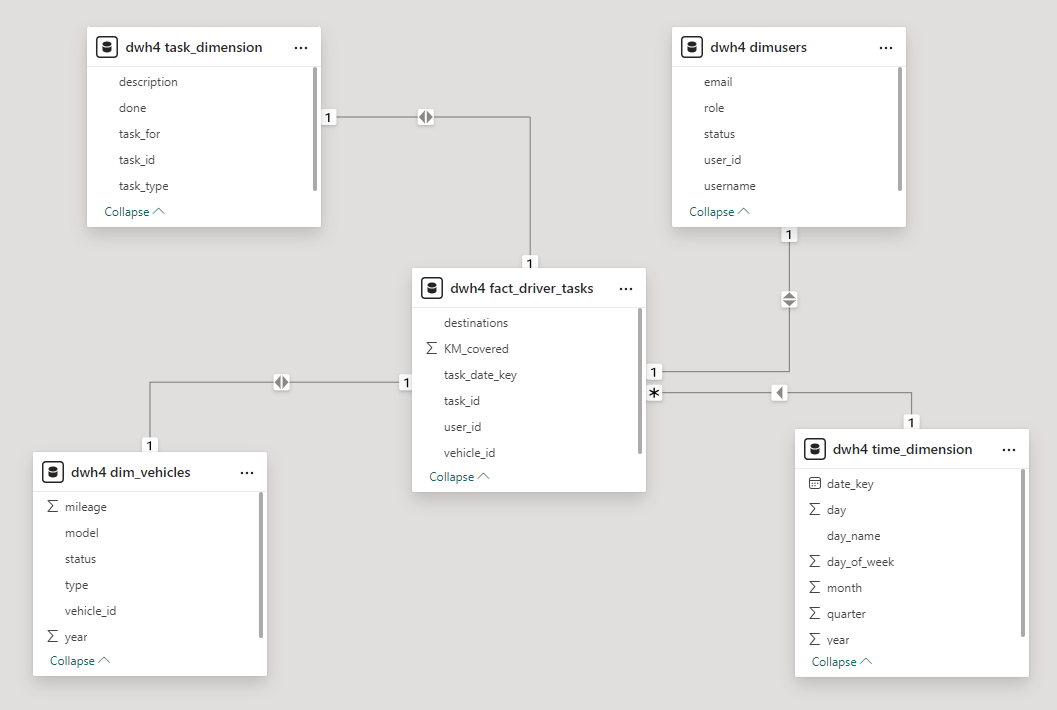
\includegraphics[width=1\textwidth,height=8cm]{chap6.images/mart driver.png}
    \caption{ Schéma en étoile : Chauffeur}

\end{figure}

\noindent
\textbf{Table de faits :} Nous utilisons la table de faits dwh4-driver-tasks-fact pour suivre et analyser les statistiques et les métriques relatives aux tâches des chauffeurs, telles que les dates des tâches, les kilomètres parcourus et les destinations associées.\\

\noindent
\textbf{Tables de dimensions utilisées:}\\
-La table de dimensions \textbf{dwh4-time-dimension} nous aide à organiser les données temporelles avec des attributs comme le jour, le mois et l'année.\\
-La table de dimensions \textbf{dwh4-dim-drivers} contient des informations sur les chauffeurs, telles que leur identifiant, leur nom d'utilisateur et leur type.\\
-La table de dimensions \textbf{dwh4-dim-vehicles} contient des informations sur les véhicules utilisés par les chauffeurs, comme le modèle, le kilométrage et le type de véhicule.\\
-La table de dimensions \textbf{dwh4-dim-destinations} contient des informations sur les destinations, avec des attributs tels que l'identifiant de la destination et le nom de la destination.\\

$\rightarrow$Avec ce datamart, nous pouvons calculer des KPI essentiels tels que le taux d'achèvement des tâches par chauffeur, les kilomètres parcourus par semaine, les tâches terminées par semaine

%_______________________________________________________________________________________________



\newpage
\section{Data mart : Véhicules}
L’objectif du data mart 'véhicules' est la gestion de la maintenance des véhicules pour garantir leur bon fonctionnement et prolonger leur durée de vie.

\subsection{ Schéma conceptuel du DataMart « Véhicules »}
\begin{figure}[h!]

    \centering
    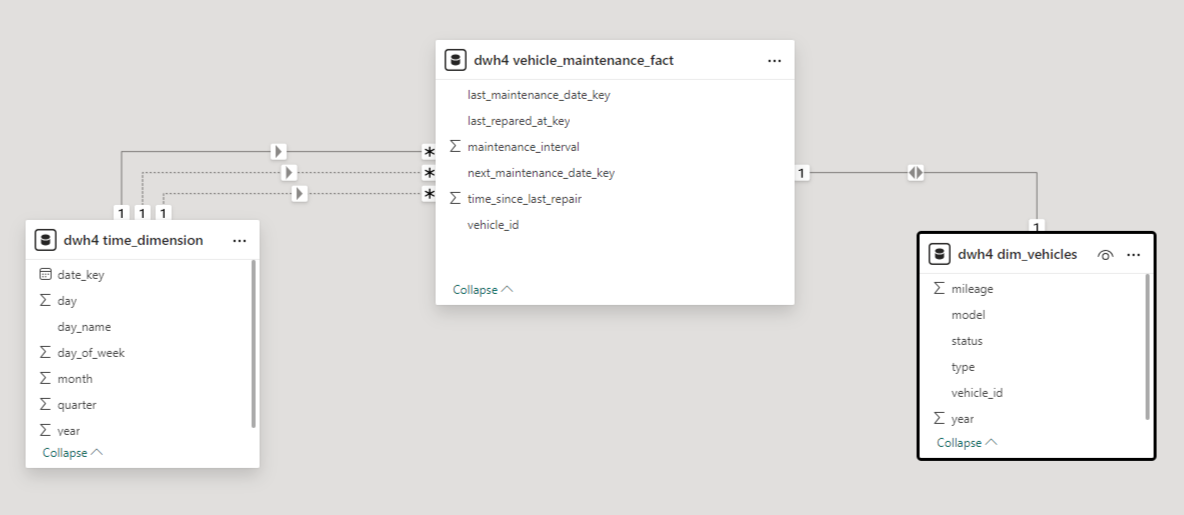
\includegraphics[width=1\textwidth, height=9cm]{chap6.images/mart vehicules.png}
    \caption{ Schéma en étoile : Véhicules}

\end{figure}

\noindent
\textbf{Table de faits :} Nous utilisons la table de faits dwh4-vehicle-maintenance-fact pour suivre et analyser les statistiques et les métriques relatives à la maintenance des véhicules, telles que les dates de maintenance et de réparation, l'intervalle de maintenance et le temps écoulé depuis la dernière réparation.\\

\noindent
\textbf{Tables de dimensions utilisées:}\\
-La table de dimensions \textbf{dwh4-time-dimension} nous aide à organiser les données temporelles avec des attributs comme le jour, le mois et l'année.\\
-La table de dimensions \textbf{dwh4-dim-vehicles} contient des informations sur les véhicules, comme -le modèle, le kilométrage et le type de véhicule.\\


$\rightarrow$Avec ce datamart, nous pouvons calculer des KPI essentiels tels que le taux de réparation des véhicules par catégorie, les kilomètres parcourus par semaine, les kilomètres par véhicule (filtrés par matricule), et le taux de panne par modèle de véhicule.




%_______________________________________________________________________________________________




\newpage
\section{Data mart : Mécanicien}
L’objectif du data mart 'Mécanicien' est le suivi et optimisation de l'exécution des tâches mécaniques.
\subsection{ Schéma conceptuel du DataMart « Mécanicien »}
\begin{figure}[h!]

    \centering
    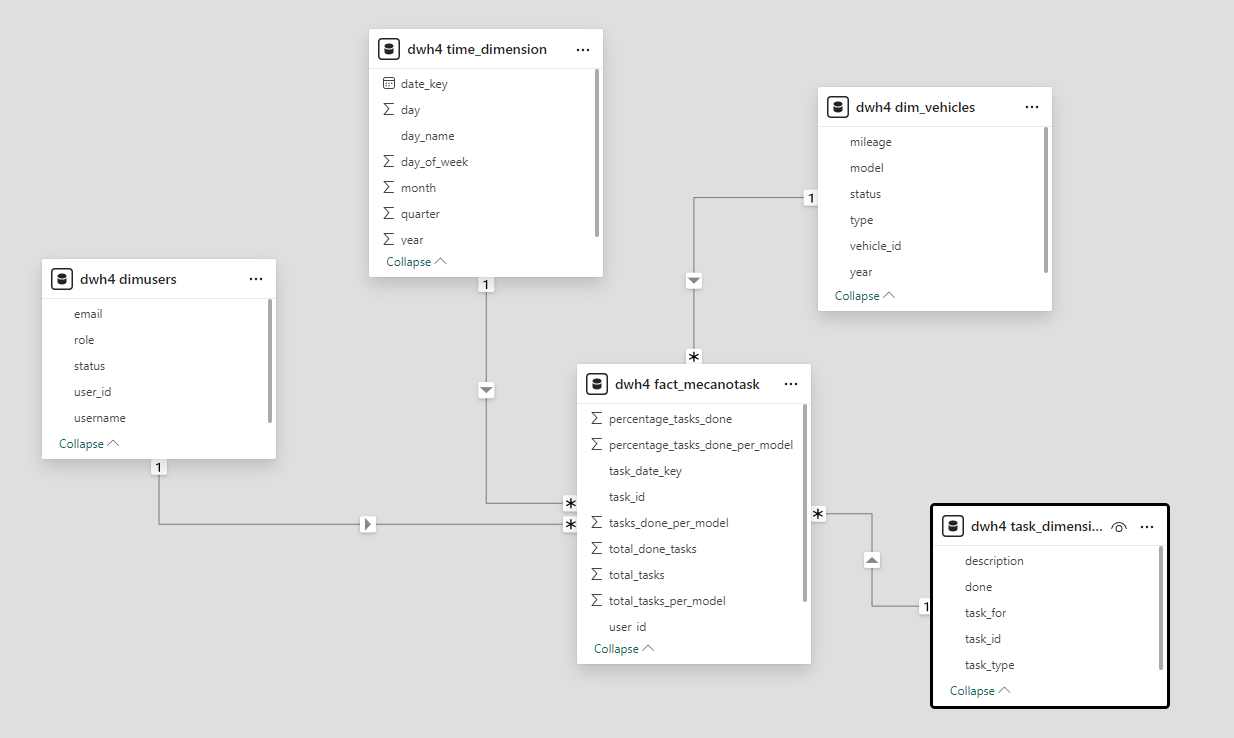
\includegraphics[width=1\textwidth, height=9cm]{chap6.images/mart mecano.png}
    \caption{ Schéma en étoile : Mécanicien}

\end{figure}
\noindent
\textbf{Table de faits :} Nous utilisons la table de faits \textbf{dwh4-fact-mecanotask} pour suivre et analyser les statistiques et les métriques relatives à l'exécution des tâches, telles que le pourcentage des tâches terminées et le nombre total de tâches terminées.\\

\noindent
\textbf{Tables de dimensions utilisées:}\\
-La table de dimensions \textbf{dwh4-time-dimension} nous aide à organiser les données temporelles avec des attributs comme le jour, le mois et l'année.\\
-La table de dimensions \textbf{dwh4-dimusers} contient des informations détaillées sur les utilisateurs, telles que leur email, leur rôle et leur statut.\\
-La table de dimensions \textbf{dwh4-dim-vehicles} contient des informations sur les véhicules, comme le modèle, le kilométrage et le type de véhicule.\\
-La table de dimensions \textbf{dwh4-task-dimension} donne des détails sur les tâches, telles que la description, le type et pour qui la tâche est destinée.\\

$\rightarrow$Avec ce datamart, nous pouvons calculer des indicateurs essentiels comme le taux d'achèvement des tâches et le nombre de tâches terminées par semaine.




%_______________________________________________________________________________________________




\newpage
\section{Data mart Utilisateurs}
L’objectif du data mart des sinistres est le Suivi de la gestion des utilisateurs et de leur engagement.

Suivi de la gestion des utilisateurs et de leur engagement.
\subsection{ Schéma conceptuel du DataMart « Utilisateurs »}
\begin{figure}[h!]

    \centering
    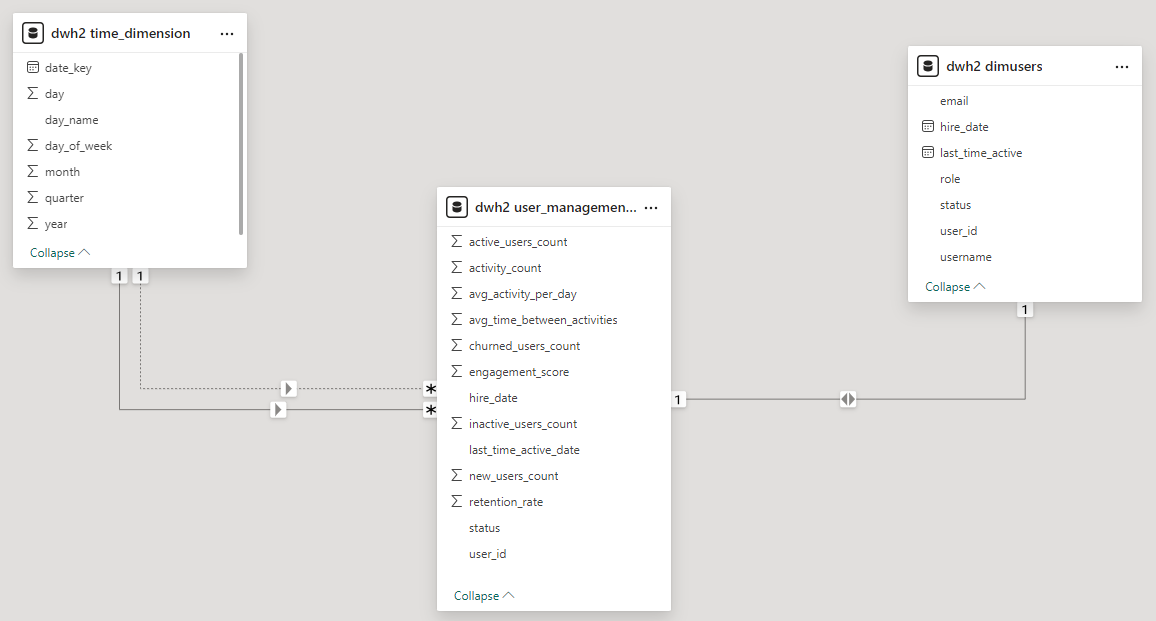
\includegraphics[width=1\textwidth]{chap6.images/etoile1.png}
    \caption{ Schéma en étoile : Utilisateurs}

\end{figure}
\noindent
\textbf{Table de faits :} Nous utilisons la table de faits \textbf{dwh2-user-management} pour suivre les statistiques et les métriques relatives aux utilisateurs, comme le nombre d'utilisateurs actifs, les activités, et le taux de rétention.\\


\noindent
\textbf{Tables de dimensions utilisées:}\\
-La table de dimensions \textbf{dwh2-time-dimension} nous aide à organiser les données temporelles avec des attributs comme le jour, le mois, et l'année.\\
-La table de dimensions \textbf{dwh2-dimusers} contient des informations détaillées sur les utilisateurs, telles que leur email, la date d'embauche, et leur rôle.\\


$\rightarrow$Avec ce datamart, nous pouvons calculer des indicateurs essentiels tels que le nombre de nouveaux utilisateurs par période et le nombre total d'utilisateurs actifs par semaine.





















%_________________________________________________________________________________________________________
\newpage
\section{Le développement de l’ETL}

L'ETL est un processus crucial en gestion des données qui consiste à extraire des données de sources variées, les transformer selon les besoins analytiques de l'entreprise, et les charger dans une structure de stockage finale comme un entrepôt de données ou un lac de données. Ce processus supporte les activités d'analyse et de prise de décision en entreprise.

\begin{figure}[h!]

    \centering
    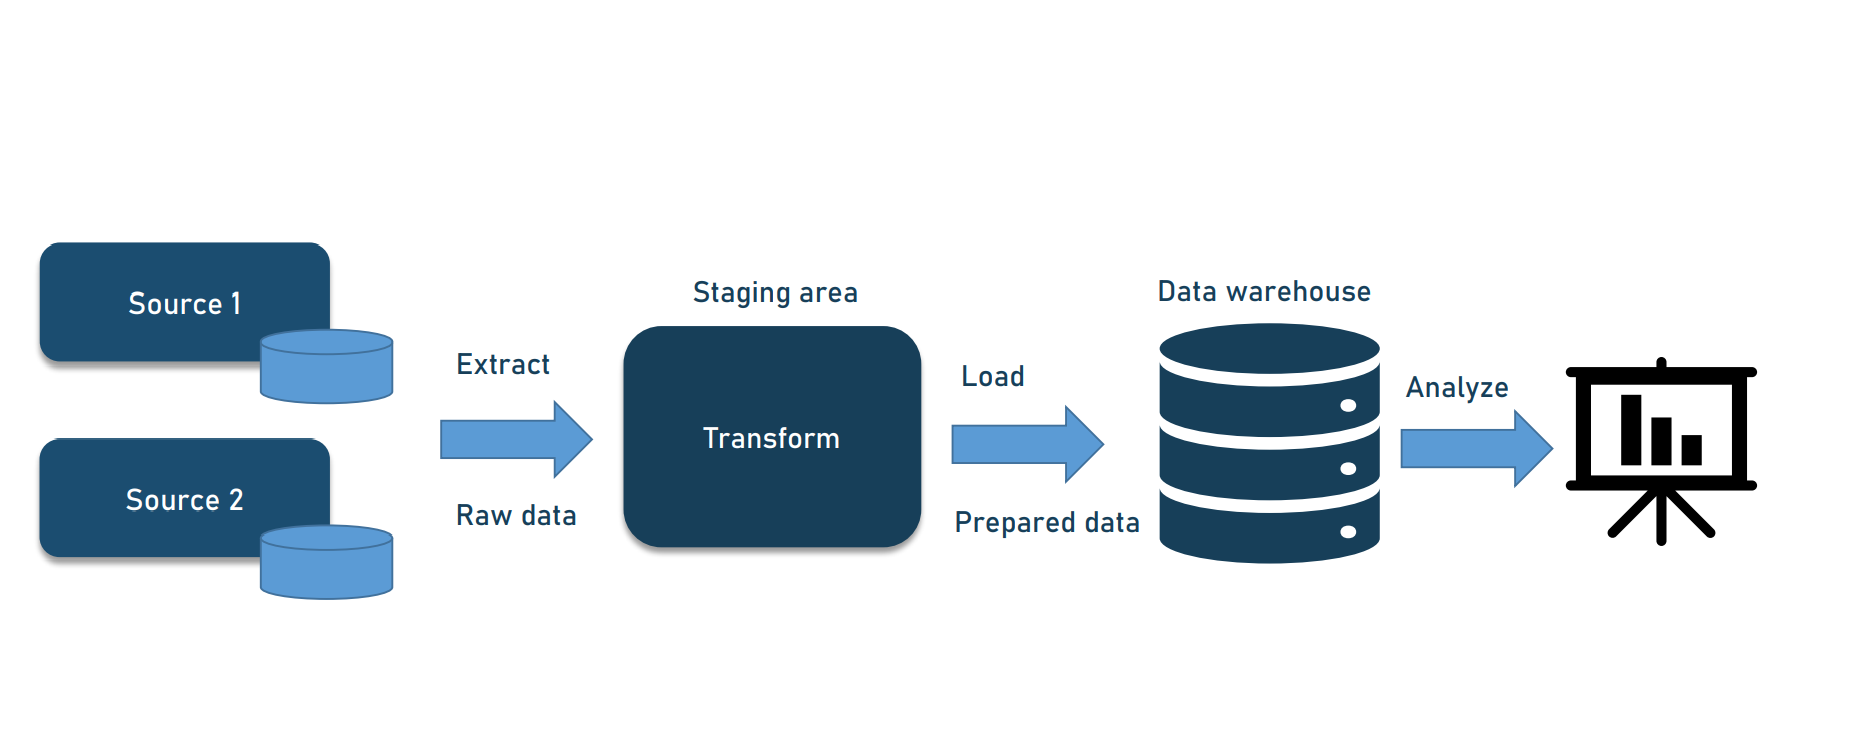
\includegraphics[width=1.05\textwidth, height=6.5cm]{chap6.images/etl-pipeline 1.png}
    \caption{ Schéma du flux de travail ETL } 


\end{figure}

\begin{itemize}



    \item[$\bullet$] \textbf {Source  :} Le source de données d'où les données sont extraites. \\
    \item[$\bullet$] \textbf {Extract :} La phase d'extraction où les données brutes sont collectées.\\
    \item[$\bullet$] \textbf {Transform :} La phase de transformation où les données sont nettoyées et transformées.\\
    \item[$\bullet$] \textbf {Load :} La phase de chargement où les données transformées sont stockées dans le Data Warehouse.\\
    \item[$\bullet$] \textbf {Data Warehouse :} Le stockage centralisé des données prêtes pour l'analyse.\\
    \item[$\bullet$] \textbf {Analyze :} L'étape finale où les données sont analysées et utilisées pour générer des insights.\\

\end{itemize}

\newpage
\subsection{Extraction des données}
L'extraction des données est la première étape du processus ETL. Le code ci-dessous montre une fonction en Python utilisée pour extraire des données d'une base de données à l'aide de la bibliothèque pandas et d'un moteur de base de données SQLAlchemy.

\begin{figure}[h!]

    \centering
    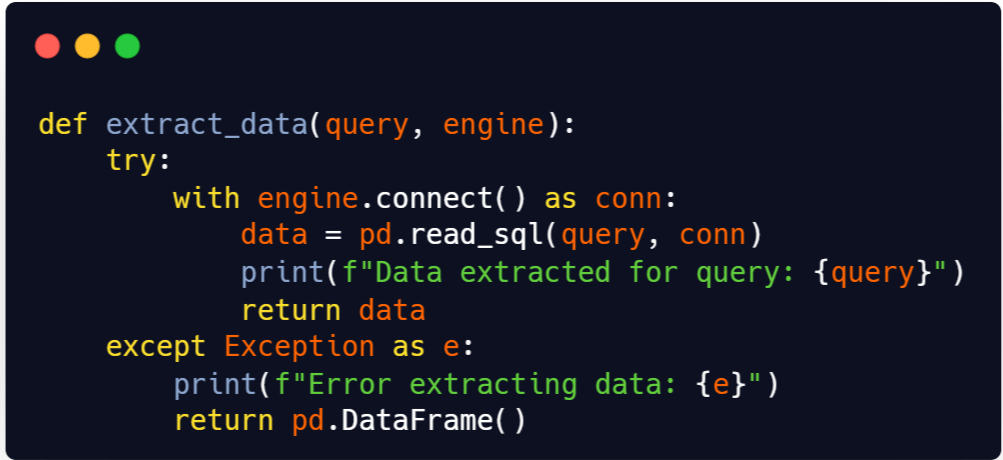
\includegraphics[width=0.9\textwidth]{chap6.images/E.png}
    \caption{ Code Source: Extraction des données}

\end{figure}

Cette fonction, extract-data, prend en entrée une requête SQL et un moteur de base de données. Elle établit une connexion à la base de données, exécute la requête SQL et charge les résultats dans un DataFrame pandas.
Cela permet de manipuler facilement les données pour les étapes suivantes. En cas d'erreur, la fonction capture l'exception et retourne un DataFrame vide, tout en affichant un message d'erreur pour faciliter le débogage.
%___________________________________________________________________________________________

\subsection{Transformation des données}
La phase de transformation du processus ETL consiste à nettoyer, enrichir et formater les données extraites pour les rendre cohérentes et prêtes à être chargées dans le Data Warehouse. Cela inclut la suppression des doublons, la correction des erreurs, la standardisation des formats et l'agrégation des données. Cette étape assure la qualité et l'intégrité des données pour les analyses futures.\\

\subsubsection{Transformation du table de dimension 'users' : transform-dim-users}
Cette fonction transforme les données des utilisateurs en renommant et en sélectionnant les colonnes nécessaires. Par exemple, elle renomme idusers en user-id, Mail en email et created-at en hire-date. Cette étape permet de standardiser les noms de colonnes pour une intégration cohérente dans le Data Warehouse.
\newpage
\begin{figure}[h!]

    \centering
    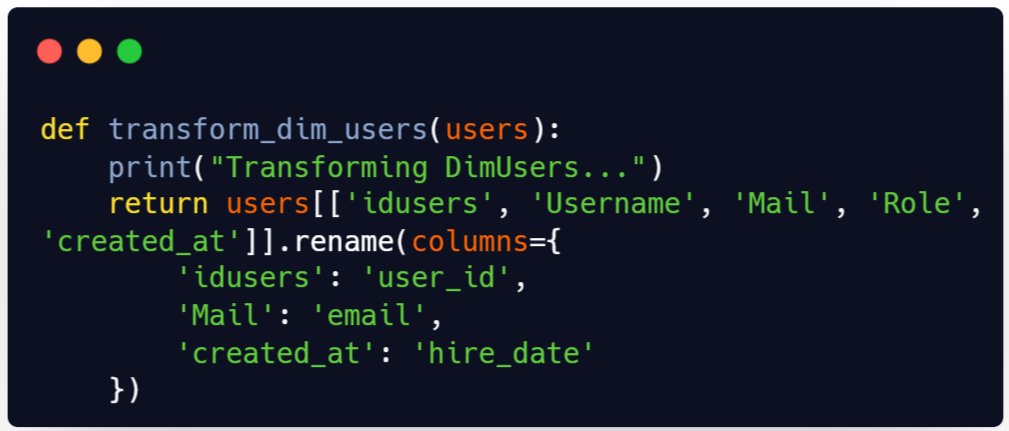
\includegraphics[width=0.9\textwidth]{chap6.images/trans users.png}
    \caption{ Transformation de la table de dimension 'users' }

\end{figure}

\subsubsection{Transformation du table de fait Tâches du chauffeur : transform-fact-driver-tasks}
Cette fonction enrichit les données des tâches des conducteurs en y intégrant les kilomètres parcourus à partir d'une autre source de données. Elle effectue une jointure et remplit les valeurs manquantes avec zéro, puis renomme et sélectionne les colonnes pour préparer les données pour le Data Warehouse.


\begin{figure}[h!]

    \centering
    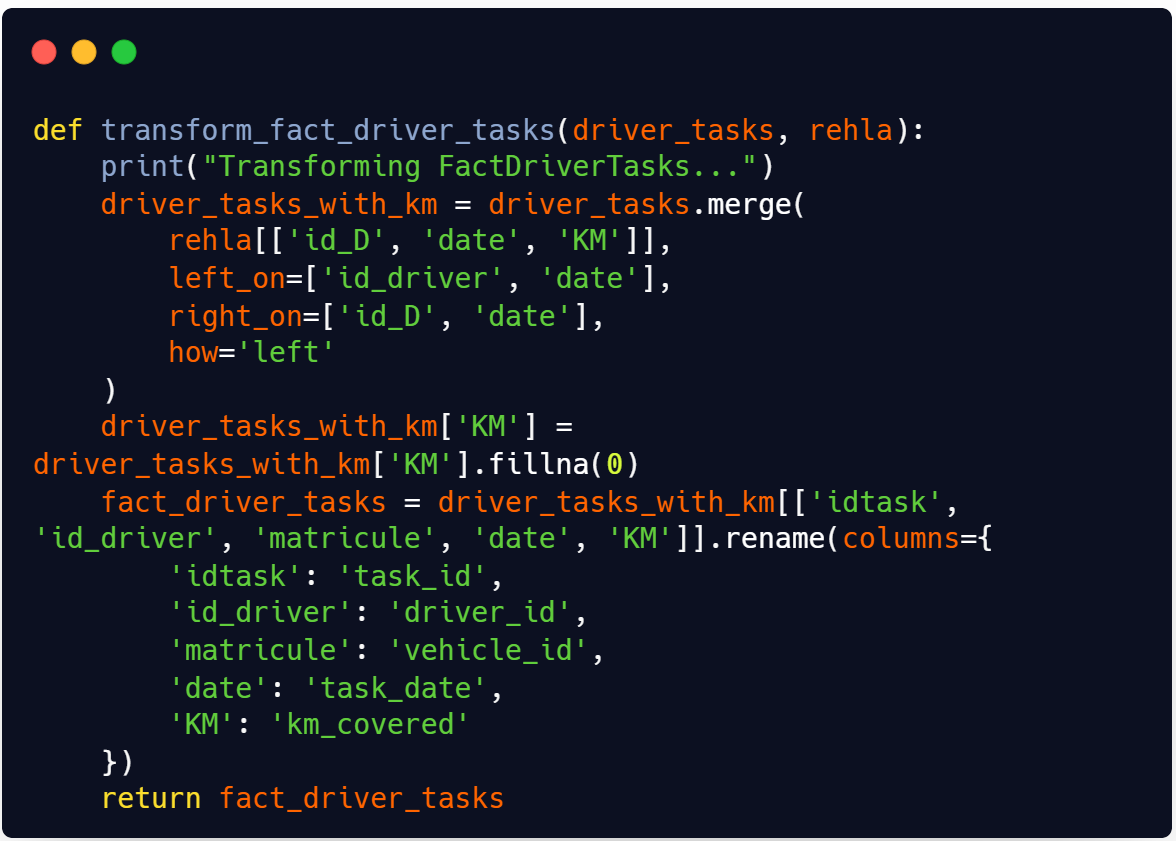
\includegraphics[width=0.9\textwidth]{chap6.images/trans fact driver task.png}
    \caption{ Transformation de la table de dimension 'users' }

\end{figure}

Ces exemples illustrent comment les données sont préparées, améliorées et structurées pour assurer leur cohérence et les rendre prêtes à être intégrées dans le Data Warehouse.

























%___________________________________________________________________________________________
\newpage
\subsection{Chargement des données}
La dernière étape du processus ETL consiste à intégrer les données extraites et transformées dans le Data Warehouse.\\

\noindent
La fonction load-data est définie avec trois paramètres : df (le DataFrame contenant les données à charger), table-name (le nom de la table cible) et engine (l'objet moteur de connexion à la base de données).\\
\textbf{Requêtes de création de table :} Un dictionnaire create-table-queries est défini pour contenir les requêtes SQL de création de tables pour chaque table cible. Ces requêtes définissent la structure de chaque table avec les colonnes et leurs types de données.\\

\subsubsection{Chargement des Données dans la Table DimUsers :}
\noindent
\textbf{-Insertion des Utilisateurs :} Les données transformées des utilisateurs, généralement stockées dans un DataFrame (df), sont insérées dans la table DimUsers. Chaque enregistrement contient les champs comme user-id, username, email, role, et hire-date.
\bigskip
\begin{figure}[h!]

    \centering
    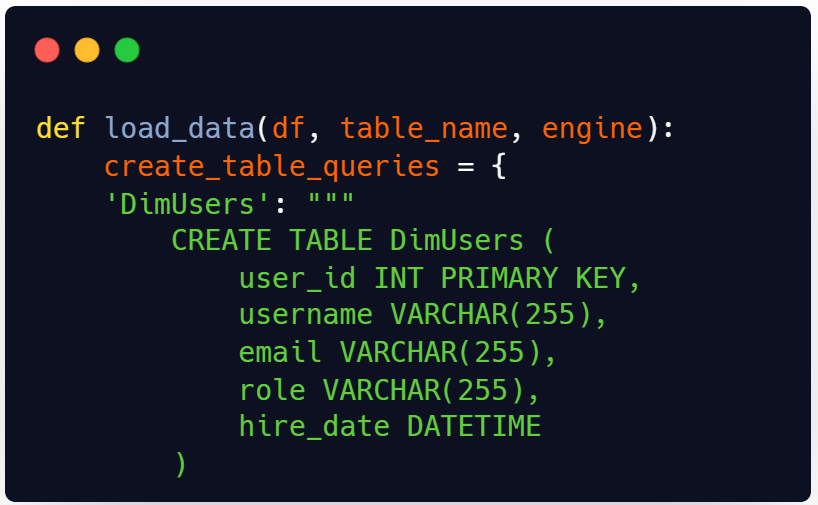
\includegraphics[width=0.7\textwidth]{chap6.images/load usee.png}
    \caption{ Chargement des Données dans la Table DimUser }

\end{figure}

Chaque utilisateur est identifié par un user-id unique et les autres champs sont utilisés pour fournir des détails importants sur chaque utilisateur.


\newpage
\subsubsection{Chargement des Données dans la Table FactDriverTasks :}
\noindent
\textbf{-Insertion des Tâches des chauffeurs :} Les données transformées des tâches des conducteurs, généralement stockées dans un DataFrame (df), sont insérées dans la table FactDriverTasks. Chaque enregistrement contient des champs comme task-id, driver-id, vehicle-id, task-date, et km-covered.

\begin{figure}[h!]

    \centering
    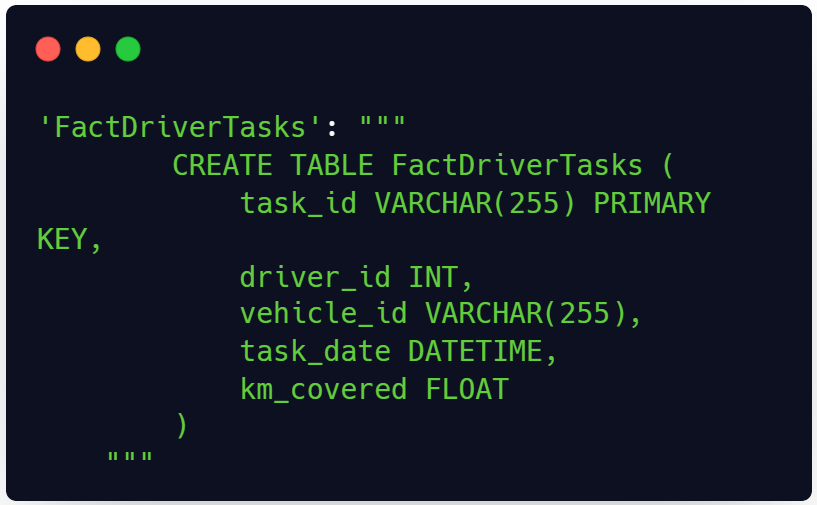
\includegraphics[width=0.7\textwidth]{chap6.images/load driver tasks.png}
    \caption{ Chargement des Données dans la Table FactDriverTasks :}

\end{figure}

Chaque tâche est identifiée par un task-id unique et les autres champs capturent des informations cruciales telles que le conducteur (driver-id), le véhicule (vehicle-id), la date de la tâche (task-date), et les kilomètres parcourus (km-covered).




















%___________________________________________________________________________________________
\newpage
\section{Choix des graphiques}

\textbf{Nivo Chart} est une bibliothèque de visualisation de données basée sur React, conçue pour créer des graphiques interactifs et réactifs. Elle offre une large gamme de types de graphiques, y compris des barres, des lignes, des pie charts, des treemaps, des heatmaps, et bien d'autres. En utilisant Nivo Chart, vous pouvez facilement créer des visualisations qui non seulement présentent les données de manière claire et attrayante, mais aussi facilitent l'interaction et l'analyse des informations. [7]\\
\bigskip
\begin{figure}[ht]
    \centering 
\includegraphics[scale=0.19]{chap6.images/nivo.png}
    \caption{Nivo Chart}
    \label{Nivo Chart}
\end{figure}

\bigskip
\noindent
Avec l'aide de Nivo Chart, nous avons opté pour les types de graphiques suivants pour représenter les différents indicateurs dans notre rapport :\\

\noindent
\textbf{Graphique en barres (Bar Chart) :} Idéal pour comparer des valeurs discrètes, notamment pour montrer le taux d'achèvement des tâches et le nombre de tâches terminées par semaine. Leur simplicité et leur lisibilité sont parfaites pour des comparaisons claires.\\


\begin{figure}[ht]
    \centering 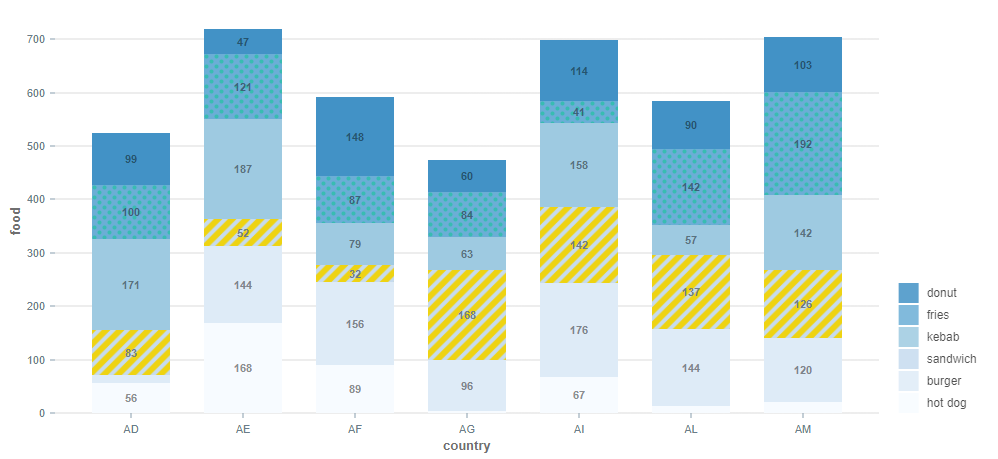
\includegraphics[scale=0.6]{chap6.images/bar.png}
    \caption{Graphique en barres}
    \label{Graphique en barres}
\end{figure}
\newpage
\noindent
\textbf{Graphique linéaire (Line Chart) :} Permet de visualiser des tendances sur une période de temps. Utilisé pour montrer l'évolution des kilomètres parcourus par semaine, mettant en évidence les variations et les tendances continues.\\

\begin{figure}[ht]
    \centering 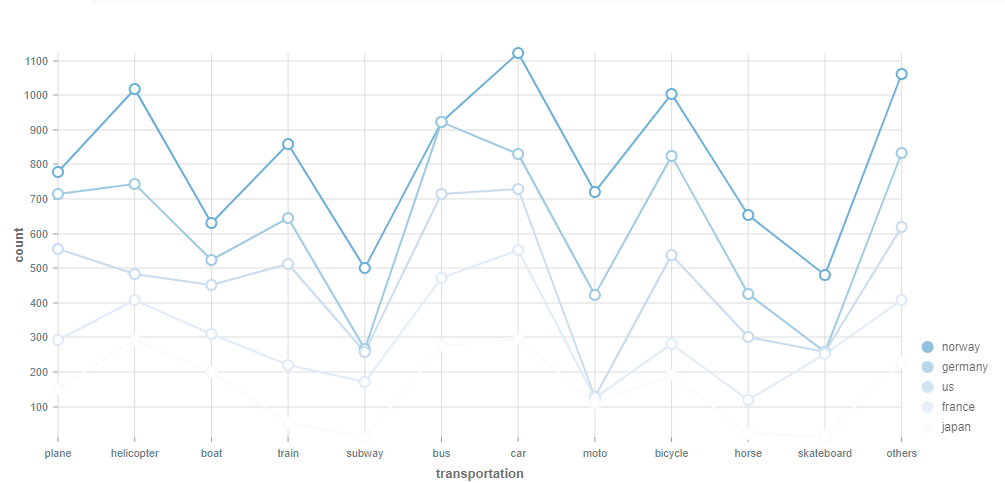
\includegraphics[scale=0.6]{chap6.images/Line.png}
    \caption{Graphique linéaire}
    \label{Graphique linéaire}
\end{figure}

\noindent
\textbf{Graphique en secteurs (Pie Chart):} Montre les proportions de différentes catégories dans un ensemble. Utile pour visualiser la répartition des types de tâches ou des pannes par catégorie de véhicule.\\

\begin{figure}[ht]
    \centering 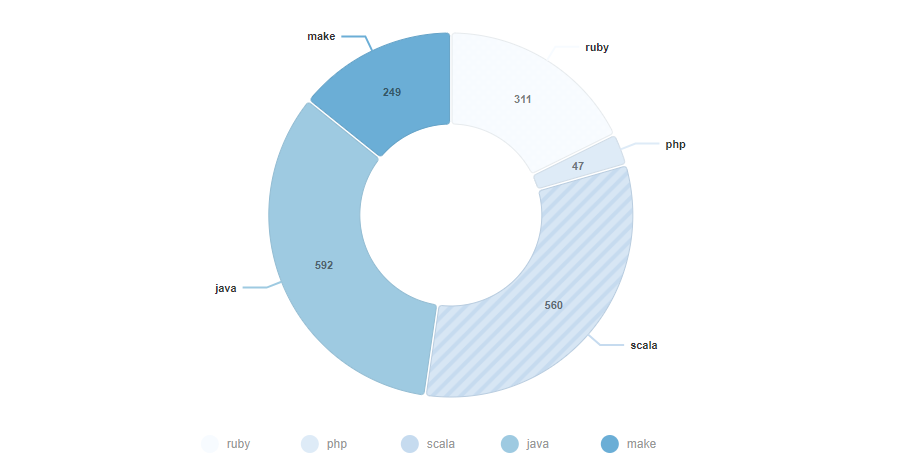
\includegraphics[scale=0.6]{chap6.images/Pie.png}
    \caption{Graphique en secteurs}
    \label{Graphique en secteurs}
\end{figure}
\newpage
\noindent
\textbf{Heatmap} : Excellente pour montrer la densité ou la fréquence d'événements dans un espace défini. Particulièrement utile pour représenter la fréquence des réparations ou l'utilisation des véhicules sur différentes périodes.

\begin{figure}[ht]
    \centering 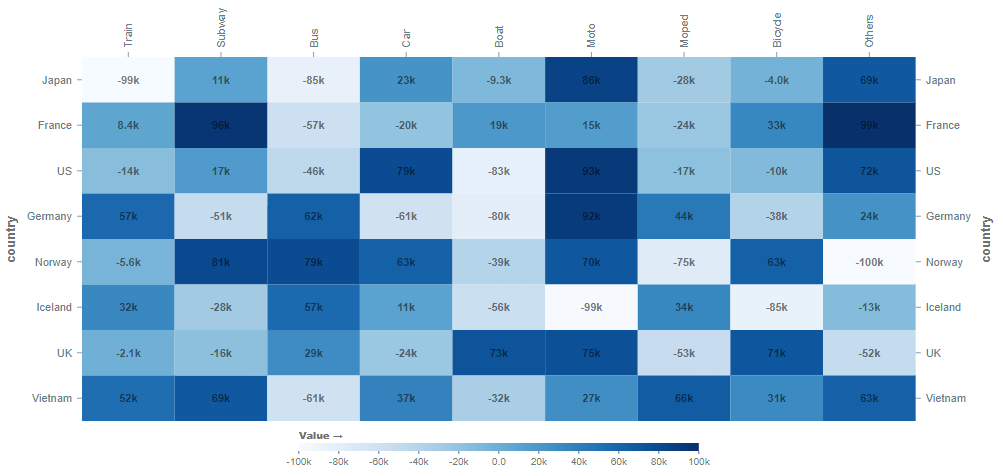
\includegraphics[scale=0.6]{chap6.images/heatmap.png}
    \caption{Heatmap}
    \label{Heatmap}
\end{figure}
\noindent
En utilisant ces différents types de graphiques, nous pouvons fournir une vue d'ensemble complète et intuitive des performances et des indicateurs clés, facilitant ainsi la prise de décision basée sur les données.
%___________________________________________________________________________________________
\newpage
\section{Publication du tableau de bord}

\subsection{Présentation des tableaux de bord  dans l'application web}
\subsection{Présentation des tableaux de bord  dans l'application mobile}

%___________________________________________________________________________________________


\section*{Conclusion}
\addcontentsline{toc}{section}{Conclusion}
Ce chapitre a décrit l'implémentation des tableaux de bord durant le sprint 4, en se concentrant sur les besoins des différents utilisateurs. Le choix d'une architecture de données adaptée a permis une gestion efficace des données et des visualisations personnalisées pour chaque profil. Les tableaux de bord créés facilitent la prise de décisions éclairées grâce à des KPI pertinents. En résumé, ce sprint a abouti à des outils analytiques robustes et essentiels pour l'amélioration continue des opérations.







